\documentclass[tikz,border=0pt]{standalone}
% The roles of Auctopus around the principal investigator: a role map, not an execution order. Each spoke is a channel
% of the orchestrator, which carries tasks from the PI to a role and documents back; the roles never message each
% other. The execution order (reviews, safety agent, human approval) is drawn in docs/workflow.md.
%   pdflatex agents.tex                                              -> agents.pdf      (light)
%   pdflatex -jobname=agents-dark "\def\darkmode{1}\documentclass[tikz,border=0pt]{standalone}
% The roles of Auctopus around the principal investigator: a role map, not an execution order. Each spoke is a channel
% of the orchestrator, which carries tasks from the PI to a role and documents back; the roles never message each
% other. The execution order (reviews, safety agent, human approval) is drawn in docs/workflow.md.
%   pdflatex agents.tex                                              -> agents.pdf      (light)
%   pdflatex -jobname=agents-dark "\def\darkmode{1}\documentclass[tikz,border=0pt]{standalone}
% The roles of Auctopus around the principal investigator: a role map, not an execution order. Each spoke is a channel
% of the orchestrator, which carries tasks from the PI to a role and documents back; the roles never message each
% other. The execution order (reviews, safety agent, human approval) is drawn in docs/workflow.md.
%   pdflatex agents.tex                                              -> agents.pdf      (light)
%   pdflatex -jobname=agents-dark "\def\darkmode{1}\documentclass[tikz,border=0pt]{standalone}
% The roles of Auctopus around the principal investigator: a role map, not an execution order. Each spoke is a channel
% of the orchestrator, which carries tasks from the PI to a role and documents back; the roles never message each
% other. The execution order (reviews, safety agent, human approval) is drawn in docs/workflow.md.
%   pdflatex agents.tex                                              -> agents.pdf      (light)
%   pdflatex -jobname=agents-dark "\def\darkmode{1}\input{agents.tex}" -> agents-dark.pdf (dark)
%   pdftocairo -svg agents.pdf ../agents.svg; pdftocairo -svg agents-dark.pdf ../agents-dark.svg
\usepackage[T1]{fontenc}
\usepackage[scaled=0.92]{helvet}
\renewcommand{\familydefault}{\sfdefault}
\usetikzlibrary{arrows.meta,backgrounds,decorations.text}
\definecolor{cblue}{RGB}{31,90,166}
\definecolor{corange}{RGB}{196,82,30}
\definecolor{claser}{RGB}{44,160,44}
\definecolor{cred}{RGB}{214,39,40}
\definecolor{cgold}{RGB}{176,125,18}
\definecolor{creview}{RGB}{122,92,158}
\ifdefined\darkmode
  \definecolor{cbg}{RGB}{13,17,23}
  \definecolor{ctext}{RGB}{230,237,243}
  \definecolor{csub}{RGB}{139,148,158}
  \definecolor{cink}{RGB}{173,186,199}
  \definecolor{cfill}{RGB}{33,38,45}
  \definecolor{cpaper}{RGB}{22,27,34}
  \definecolor{cring}{RGB}{110,118,129}
  \colorlet{cask}{black!20!white}
  \colorlet{cprove}{cblue!55!white}
  \colorlet{cmeasure}{claser!75!white}
  \colorlet{cdesign}{cgold!80!white}
  \colorlet{creviewc}{creview!65!white}
  \colorlet{csafe}{black!12!white}
\else
  \definecolor{cbg}{RGB}{255,255,255}
  \definecolor{ctext}{RGB}{50,52,56}
  \definecolor{csub}{RGB}{101,109,118}
  \definecolor{cink}{RGB}{50,52,56}
  \definecolor{cfill}{RGB}{243,244,246}
  \definecolor{cpaper}{RGB}{255,255,255}
  \definecolor{cring}{RGB}{150,155,160}
  \colorlet{cask}{black!55}
  \colorlet{cprove}{cblue}
  \colorlet{cmeasure}{claser!75!black}
  \colorlet{cdesign}{cgold}
  \colorlet{creviewc}{creview}
  \colorlet{csafe}{black!78}
\fi
\begin{document}
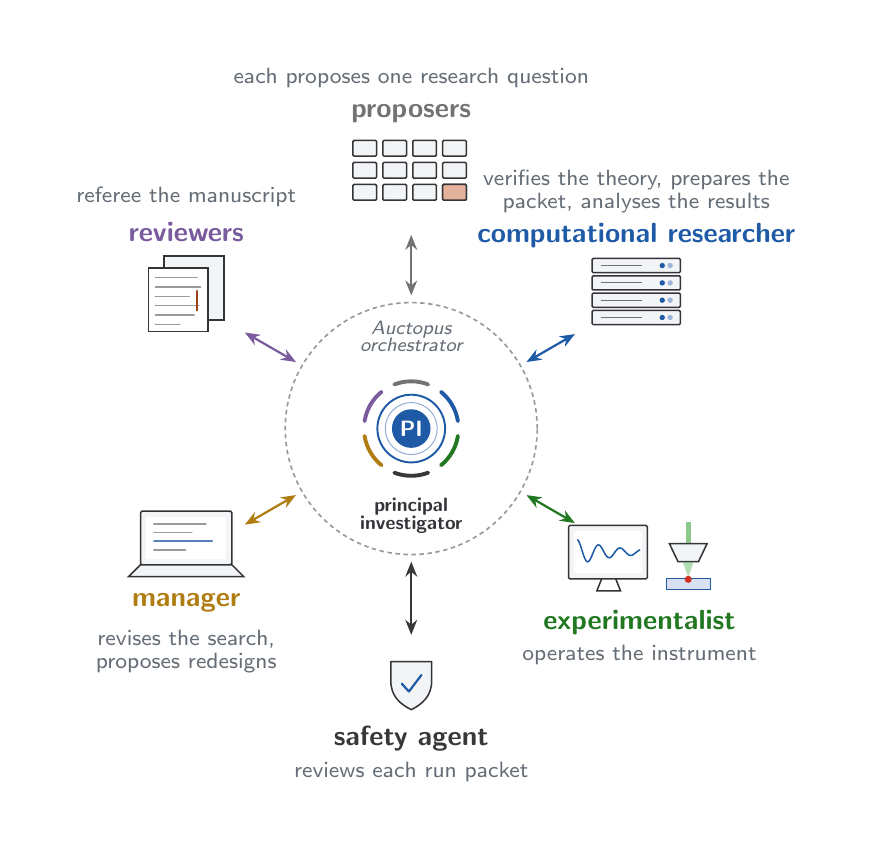
\begin{tikzpicture}[x=1mm, y=1mm,
  show background rectangle, inner frame xsep=5mm, inner frame ysep=4mm,
  background rectangle/.style={fill=cbg, rounded corners=3mm},
  ink/.style={draw=cink, line width=0.55pt},
  name/.style={font=\normalsize\bfseries, align=center},
  does/.style={font=\footnotesize, text=csub, align=center},
  spoke/.style={line width=0.8pt, {Stealth[length=1.9mm,width=1.5mm]}-{Stealth[length=1.9mm,width=1.5mm]}}]

\def\R{33}     % centre of each role's icon
\def\ring{16}  % the orchestrator

% ---------- the orchestrator: a ring around the PI, one spoke per role ----------
\draw[cring, line width=0.6pt, dash pattern=on 1.6pt off 1.3pt] (0,0) circle (\ring);
\node[does, font=\scriptsize\itshape, anchor=south] at (0,8.6) {Auctopus\\[-2pt]orchestrator};
\foreach \a/\c/\r in {90/cask/24.6, 30/cprove/24.0, -30/cmeasure/24.0, -90/csafe/26.2, -150/cdesign/24.4,
                      150/creviewc/24.4} {
  \draw[spoke, \c] (\a:\ring+0.9) -- (\a:\r);
}

% ---------- the principal investigator ----------
\foreach \a/\c in {90/cask, 30/cprove, -30/cmeasure, -90/csafe, -150/cdesign, 150/creviewc} {
  \draw[\c, line width=1.4pt, line cap=round] (\a-21:6.0) arc[start angle=\a-21, end angle=\a+21, radius=6.0];
}
\filldraw[draw=cblue, line width=0.7pt, fill=cpaper] (0,0) circle (4.3);
\draw[cblue!50, line width=0.35pt] (0,0) circle (3.3);
\fill[cblue] (0,0) circle (2.45);
\node[text=white, font=\footnotesize\bfseries, inner sep=0pt] at (0,0) {PI};
\node[name, text=ctext, font=\scriptsize\bfseries, anchor=north] at (0,-7.6) {principal\\[-1.5pt]investigator};

% ---------- proposers (top) ----------
\begin{scope}[shift={(90:\R)}]
  \foreach \i in {0,...,3} {\foreach \j in {0,...,2} {
    \filldraw[ink, fill=cfill, rounded corners=0.4pt] ({-7.4+\i*3.8},{-4.0+\j*2.8}) rectangle ++(3.0,2.0);
  }}
  \filldraw[ink, fill=corange!45, rounded corners=0.4pt] ({-7.4+3*3.8},{-4.0}) rectangle ++(3.0,2.0);
  \node[name, text=cask, anchor=south] at (0,4.6) {proposers};
  \node[does, anchor=south] at (0,9.0) {each proposes one research question};
\end{scope}

% ---------- computational researcher (upper right) ----------
\begin{scope}[shift={(30:\R)}]
  \foreach \k in {0,...,3} {
    \filldraw[ink, fill=cfill, rounded corners=0.4pt] (-5.6,{-3.3+2.2*\k}) rectangle (5.6,{-1.5+2.2*\k});
    \draw[cink!70, line width=0.35pt] (-4.5,{-2.4+2.2*\k}) -- (0.7,{-2.4+2.2*\k});
    \fill[cblue] (3.3,{-2.4+2.2*\k}) circle (0.34);
    \fill[cblue!45] (4.3,{-2.4+2.2*\k}) circle (0.34);
  }
  \node[name, text=cprove, anchor=south] at (0,5.2) {computational researcher};
  \node[does, anchor=south] at (0,9.6) {verifies the theory, prepares the\\[-1pt] packet, analyses the results};
\end{scope}

% ---------- experimentalist (lower right) ----------
\begin{scope}[shift={(-30:\R)}]
  \filldraw[ink, fill=cfill, rounded corners=0.5pt] (-8.6,-2.6) rectangle (1.4,4.2);
  \fill[cpaper] (-7.9,-1.9) rectangle (0.7,3.5);
  \draw[cblue, line width=0.55pt, domain=0:8.0, samples=60, smooth]
       plot ({-7.5+\x}, {0.8+1.6*exp(-0.2*\x)*cos(deg(2.3*\x))});
  \draw[ink] (-4.4,-2.6) -- (-5.0,-4.1) -- (-2.0,-4.1) -- (-2.6,-2.6);
  \fill[claser, opacity=0.55] (6.3,4.6) rectangle (6.9,1.9);
  \filldraw[ink, fill=cfill] (4.2,1.9) -- (9.0,1.9) -- (7.9,-0.4) -- (5.3,-0.4) -- cycle;
  \fill[claser, opacity=0.35] (5.9,-0.4) -- (7.3,-0.4) -- (6.6,-2.4) -- cycle;
  \filldraw[draw=cblue, line width=0.45pt, fill=cblue!18] (3.8,-3.9) rectangle (9.4,-2.5);
  \fill[cred!75!corange] (6.6,-2.65) circle (0.45);
  \node[name, text=cmeasure, anchor=north] at (0.4,-5.3) {experimentalist};
  \node[does, anchor=north] at (0.4,-9.8) {operates the instrument};
\end{scope}

% ---------- safety agent (bottom) ----------
\begin{scope}[shift={(-90:\R)}]
  \filldraw[ink, fill=cfill, line join=round] (-2.6,3.4) -- (2.6,3.4) -- (2.6,1.0)
       .. controls (2.6,-1.0) and (1.4,-2.0) .. (0,-2.7) .. controls (-1.4,-2.0) and (-2.6,-1.0) .. (-2.6,1.0) -- cycle;
  \draw[cblue, line width=0.8pt, line cap=round, line join=round] (-1.2,0.6) -- (-0.3,-0.4) -- (1.3,1.7);
  \node[name, text=csafe, anchor=north] at (0,-3.6) {safety agent};
  \node[does, anchor=north] at (0,-8.1) {reviews each run packet};
\end{scope}

% ---------- manager (lower left) ----------
\begin{scope}[shift={(-150:\R)}]
  \filldraw[ink, fill=cfill, rounded corners=0.5pt] (-5.8,-0.8) rectangle (5.8,6.0);
  \fill[cpaper] (-5.1,-0.1) rectangle (5.1,5.3);
  \foreach \y/\l/\c in {4.4/6.6/cring, 3.3/4.8/cring, 2.2/7.4/cblue!75, 1.1/4.0/cring} {
    \draw[\c, line width=0.6pt, line cap=round] (-4.1,\y) -- (-4.1+\l,\y);
  }
  \filldraw[ink, fill=cfill] (-7.3,-2.3) -- (7.3,-2.3) -- (5.8,-0.8) -- (-5.8,-0.8) -- cycle;
  \node[name, text=cdesign, anchor=north] at (0,-3.3) {manager};
  \node[does, anchor=north] at (0,-7.8) {revises the search,\\[-1pt] proposes redesigns};
\end{scope}

% ---------- reviewers (upper left) ----------
\begin{scope}[shift={(150:\R)}]
  \filldraw[ink, fill=cfill] (-2.8,-2.7) rectangle (4.8,5.4);
  \filldraw[ink, fill=cpaper] (-4.8,-4.2) rectangle (2.8,3.9);
  \foreach \y/\l in {2.7/5.3, 1.5/5.7, 0.3/4.3, -0.9/5.5, -2.1/4.9, -3.3/3.1} {
    \draw[cring, line width=0.55pt, line cap=round] (-3.9,\y) -- (-3.9+\l,\y);
  }
  \draw[corange!80!black, line width=0.7pt, line cap=round] (1.4,1.0) -- (1.4,-1.5);
  \node[name, text=creviewc, anchor=south] at (0,6.0) {reviewers};
  \node[does, anchor=south] at (0,10.4) {referee the manuscript};
\end{scope}

\end{tikzpicture}
\end{document}
" -> agents-dark.pdf (dark)
%   pdftocairo -svg agents.pdf ../agents.svg; pdftocairo -svg agents-dark.pdf ../agents-dark.svg
\usepackage[T1]{fontenc}
\usepackage[scaled=0.92]{helvet}
\renewcommand{\familydefault}{\sfdefault}
\usetikzlibrary{arrows.meta,backgrounds,decorations.text}
\definecolor{cblue}{RGB}{31,90,166}
\definecolor{corange}{RGB}{196,82,30}
\definecolor{claser}{RGB}{44,160,44}
\definecolor{cred}{RGB}{214,39,40}
\definecolor{cgold}{RGB}{176,125,18}
\definecolor{creview}{RGB}{122,92,158}
\ifdefined\darkmode
  \definecolor{cbg}{RGB}{13,17,23}
  \definecolor{ctext}{RGB}{230,237,243}
  \definecolor{csub}{RGB}{139,148,158}
  \definecolor{cink}{RGB}{173,186,199}
  \definecolor{cfill}{RGB}{33,38,45}
  \definecolor{cpaper}{RGB}{22,27,34}
  \definecolor{cring}{RGB}{110,118,129}
  \colorlet{cask}{black!20!white}
  \colorlet{cprove}{cblue!55!white}
  \colorlet{cmeasure}{claser!75!white}
  \colorlet{cdesign}{cgold!80!white}
  \colorlet{creviewc}{creview!65!white}
  \colorlet{csafe}{black!12!white}
\else
  \definecolor{cbg}{RGB}{255,255,255}
  \definecolor{ctext}{RGB}{50,52,56}
  \definecolor{csub}{RGB}{101,109,118}
  \definecolor{cink}{RGB}{50,52,56}
  \definecolor{cfill}{RGB}{243,244,246}
  \definecolor{cpaper}{RGB}{255,255,255}
  \definecolor{cring}{RGB}{150,155,160}
  \colorlet{cask}{black!55}
  \colorlet{cprove}{cblue}
  \colorlet{cmeasure}{claser!75!black}
  \colorlet{cdesign}{cgold}
  \colorlet{creviewc}{creview}
  \colorlet{csafe}{black!78}
\fi
\begin{document}
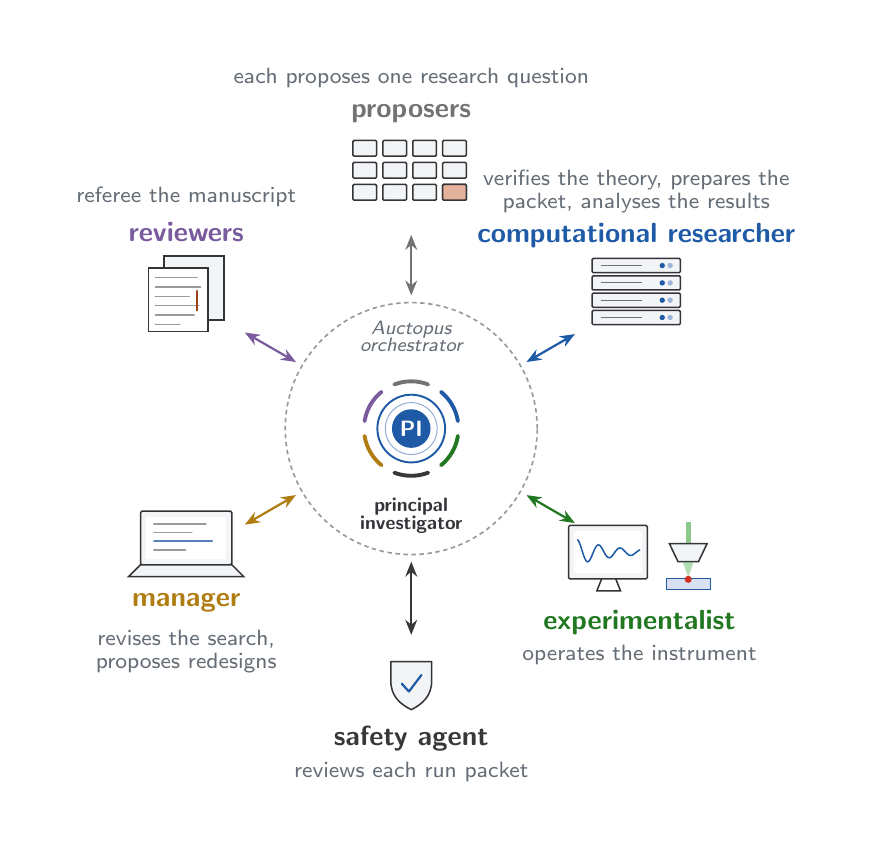
\begin{tikzpicture}[x=1mm, y=1mm,
  show background rectangle, inner frame xsep=5mm, inner frame ysep=4mm,
  background rectangle/.style={fill=cbg, rounded corners=3mm},
  ink/.style={draw=cink, line width=0.55pt},
  name/.style={font=\normalsize\bfseries, align=center},
  does/.style={font=\footnotesize, text=csub, align=center},
  spoke/.style={line width=0.8pt, {Stealth[length=1.9mm,width=1.5mm]}-{Stealth[length=1.9mm,width=1.5mm]}}]

\def\R{33}     % centre of each role's icon
\def\ring{16}  % the orchestrator

% ---------- the orchestrator: a ring around the PI, one spoke per role ----------
\draw[cring, line width=0.6pt, dash pattern=on 1.6pt off 1.3pt] (0,0) circle (\ring);
\node[does, font=\scriptsize\itshape, anchor=south] at (0,8.6) {Auctopus\\[-2pt]orchestrator};
\foreach \a/\c/\r in {90/cask/24.6, 30/cprove/24.0, -30/cmeasure/24.0, -90/csafe/26.2, -150/cdesign/24.4,
                      150/creviewc/24.4} {
  \draw[spoke, \c] (\a:\ring+0.9) -- (\a:\r);
}

% ---------- the principal investigator ----------
\foreach \a/\c in {90/cask, 30/cprove, -30/cmeasure, -90/csafe, -150/cdesign, 150/creviewc} {
  \draw[\c, line width=1.4pt, line cap=round] (\a-21:6.0) arc[start angle=\a-21, end angle=\a+21, radius=6.0];
}
\filldraw[draw=cblue, line width=0.7pt, fill=cpaper] (0,0) circle (4.3);
\draw[cblue!50, line width=0.35pt] (0,0) circle (3.3);
\fill[cblue] (0,0) circle (2.45);
\node[text=white, font=\footnotesize\bfseries, inner sep=0pt] at (0,0) {PI};
\node[name, text=ctext, font=\scriptsize\bfseries, anchor=north] at (0,-7.6) {principal\\[-1.5pt]investigator};

% ---------- proposers (top) ----------
\begin{scope}[shift={(90:\R)}]
  \foreach \i in {0,...,3} {\foreach \j in {0,...,2} {
    \filldraw[ink, fill=cfill, rounded corners=0.4pt] ({-7.4+\i*3.8},{-4.0+\j*2.8}) rectangle ++(3.0,2.0);
  }}
  \filldraw[ink, fill=corange!45, rounded corners=0.4pt] ({-7.4+3*3.8},{-4.0}) rectangle ++(3.0,2.0);
  \node[name, text=cask, anchor=south] at (0,4.6) {proposers};
  \node[does, anchor=south] at (0,9.0) {each proposes one research question};
\end{scope}

% ---------- computational researcher (upper right) ----------
\begin{scope}[shift={(30:\R)}]
  \foreach \k in {0,...,3} {
    \filldraw[ink, fill=cfill, rounded corners=0.4pt] (-5.6,{-3.3+2.2*\k}) rectangle (5.6,{-1.5+2.2*\k});
    \draw[cink!70, line width=0.35pt] (-4.5,{-2.4+2.2*\k}) -- (0.7,{-2.4+2.2*\k});
    \fill[cblue] (3.3,{-2.4+2.2*\k}) circle (0.34);
    \fill[cblue!45] (4.3,{-2.4+2.2*\k}) circle (0.34);
  }
  \node[name, text=cprove, anchor=south] at (0,5.2) {computational researcher};
  \node[does, anchor=south] at (0,9.6) {verifies the theory, prepares the\\[-1pt] packet, analyses the results};
\end{scope}

% ---------- experimentalist (lower right) ----------
\begin{scope}[shift={(-30:\R)}]
  \filldraw[ink, fill=cfill, rounded corners=0.5pt] (-8.6,-2.6) rectangle (1.4,4.2);
  \fill[cpaper] (-7.9,-1.9) rectangle (0.7,3.5);
  \draw[cblue, line width=0.55pt, domain=0:8.0, samples=60, smooth]
       plot ({-7.5+\x}, {0.8+1.6*exp(-0.2*\x)*cos(deg(2.3*\x))});
  \draw[ink] (-4.4,-2.6) -- (-5.0,-4.1) -- (-2.0,-4.1) -- (-2.6,-2.6);
  \fill[claser, opacity=0.55] (6.3,4.6) rectangle (6.9,1.9);
  \filldraw[ink, fill=cfill] (4.2,1.9) -- (9.0,1.9) -- (7.9,-0.4) -- (5.3,-0.4) -- cycle;
  \fill[claser, opacity=0.35] (5.9,-0.4) -- (7.3,-0.4) -- (6.6,-2.4) -- cycle;
  \filldraw[draw=cblue, line width=0.45pt, fill=cblue!18] (3.8,-3.9) rectangle (9.4,-2.5);
  \fill[cred!75!corange] (6.6,-2.65) circle (0.45);
  \node[name, text=cmeasure, anchor=north] at (0.4,-5.3) {experimentalist};
  \node[does, anchor=north] at (0.4,-9.8) {operates the instrument};
\end{scope}

% ---------- safety agent (bottom) ----------
\begin{scope}[shift={(-90:\R)}]
  \filldraw[ink, fill=cfill, line join=round] (-2.6,3.4) -- (2.6,3.4) -- (2.6,1.0)
       .. controls (2.6,-1.0) and (1.4,-2.0) .. (0,-2.7) .. controls (-1.4,-2.0) and (-2.6,-1.0) .. (-2.6,1.0) -- cycle;
  \draw[cblue, line width=0.8pt, line cap=round, line join=round] (-1.2,0.6) -- (-0.3,-0.4) -- (1.3,1.7);
  \node[name, text=csafe, anchor=north] at (0,-3.6) {safety agent};
  \node[does, anchor=north] at (0,-8.1) {reviews each run packet};
\end{scope}

% ---------- manager (lower left) ----------
\begin{scope}[shift={(-150:\R)}]
  \filldraw[ink, fill=cfill, rounded corners=0.5pt] (-5.8,-0.8) rectangle (5.8,6.0);
  \fill[cpaper] (-5.1,-0.1) rectangle (5.1,5.3);
  \foreach \y/\l/\c in {4.4/6.6/cring, 3.3/4.8/cring, 2.2/7.4/cblue!75, 1.1/4.0/cring} {
    \draw[\c, line width=0.6pt, line cap=round] (-4.1,\y) -- (-4.1+\l,\y);
  }
  \filldraw[ink, fill=cfill] (-7.3,-2.3) -- (7.3,-2.3) -- (5.8,-0.8) -- (-5.8,-0.8) -- cycle;
  \node[name, text=cdesign, anchor=north] at (0,-3.3) {manager};
  \node[does, anchor=north] at (0,-7.8) {revises the search,\\[-1pt] proposes redesigns};
\end{scope}

% ---------- reviewers (upper left) ----------
\begin{scope}[shift={(150:\R)}]
  \filldraw[ink, fill=cfill] (-2.8,-2.7) rectangle (4.8,5.4);
  \filldraw[ink, fill=cpaper] (-4.8,-4.2) rectangle (2.8,3.9);
  \foreach \y/\l in {2.7/5.3, 1.5/5.7, 0.3/4.3, -0.9/5.5, -2.1/4.9, -3.3/3.1} {
    \draw[cring, line width=0.55pt, line cap=round] (-3.9,\y) -- (-3.9+\l,\y);
  }
  \draw[corange!80!black, line width=0.7pt, line cap=round] (1.4,1.0) -- (1.4,-1.5);
  \node[name, text=creviewc, anchor=south] at (0,6.0) {reviewers};
  \node[does, anchor=south] at (0,10.4) {referee the manuscript};
\end{scope}

\end{tikzpicture}
\end{document}
" -> agents-dark.pdf (dark)
%   pdftocairo -svg agents.pdf ../agents.svg; pdftocairo -svg agents-dark.pdf ../agents-dark.svg
\usepackage[T1]{fontenc}
\usepackage[scaled=0.92]{helvet}
\renewcommand{\familydefault}{\sfdefault}
\usetikzlibrary{arrows.meta,backgrounds,decorations.text}
\definecolor{cblue}{RGB}{31,90,166}
\definecolor{corange}{RGB}{196,82,30}
\definecolor{claser}{RGB}{44,160,44}
\definecolor{cred}{RGB}{214,39,40}
\definecolor{cgold}{RGB}{176,125,18}
\definecolor{creview}{RGB}{122,92,158}
\ifdefined\darkmode
  \definecolor{cbg}{RGB}{13,17,23}
  \definecolor{ctext}{RGB}{230,237,243}
  \definecolor{csub}{RGB}{139,148,158}
  \definecolor{cink}{RGB}{173,186,199}
  \definecolor{cfill}{RGB}{33,38,45}
  \definecolor{cpaper}{RGB}{22,27,34}
  \definecolor{cring}{RGB}{110,118,129}
  \colorlet{cask}{black!20!white}
  \colorlet{cprove}{cblue!55!white}
  \colorlet{cmeasure}{claser!75!white}
  \colorlet{cdesign}{cgold!80!white}
  \colorlet{creviewc}{creview!65!white}
  \colorlet{csafe}{black!12!white}
\else
  \definecolor{cbg}{RGB}{255,255,255}
  \definecolor{ctext}{RGB}{50,52,56}
  \definecolor{csub}{RGB}{101,109,118}
  \definecolor{cink}{RGB}{50,52,56}
  \definecolor{cfill}{RGB}{243,244,246}
  \definecolor{cpaper}{RGB}{255,255,255}
  \definecolor{cring}{RGB}{150,155,160}
  \colorlet{cask}{black!55}
  \colorlet{cprove}{cblue}
  \colorlet{cmeasure}{claser!75!black}
  \colorlet{cdesign}{cgold}
  \colorlet{creviewc}{creview}
  \colorlet{csafe}{black!78}
\fi
\begin{document}
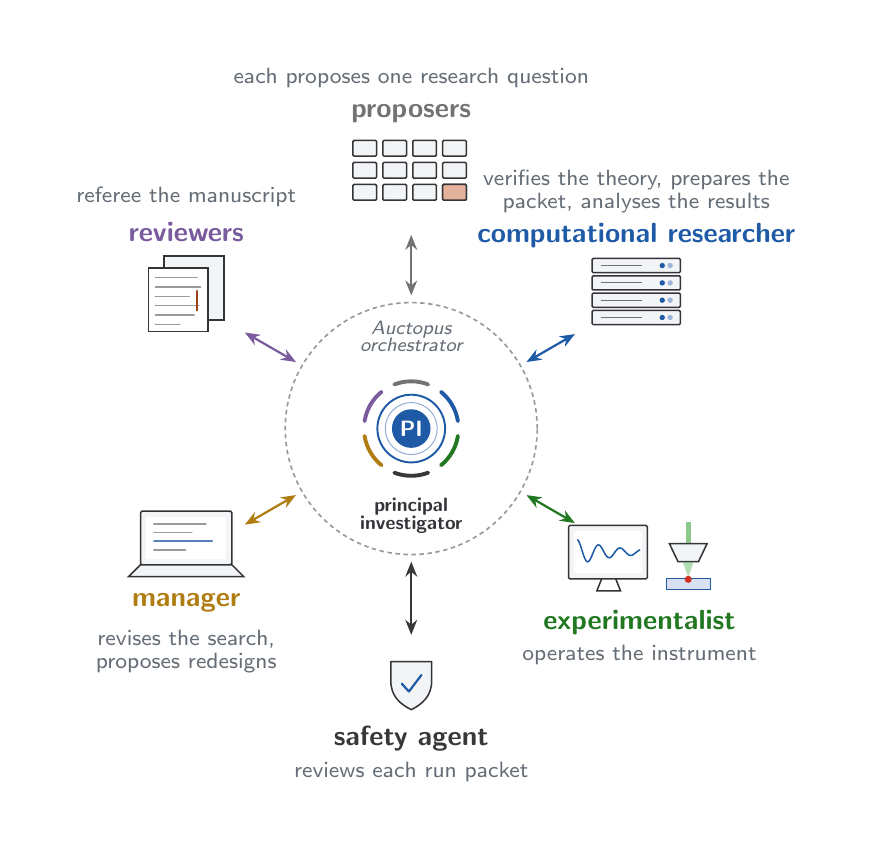
\begin{tikzpicture}[x=1mm, y=1mm,
  show background rectangle, inner frame xsep=5mm, inner frame ysep=4mm,
  background rectangle/.style={fill=cbg, rounded corners=3mm},
  ink/.style={draw=cink, line width=0.55pt},
  name/.style={font=\normalsize\bfseries, align=center},
  does/.style={font=\footnotesize, text=csub, align=center},
  spoke/.style={line width=0.8pt, {Stealth[length=1.9mm,width=1.5mm]}-{Stealth[length=1.9mm,width=1.5mm]}}]

\def\R{33}     % centre of each role's icon
\def\ring{16}  % the orchestrator

% ---------- the orchestrator: a ring around the PI, one spoke per role ----------
\draw[cring, line width=0.6pt, dash pattern=on 1.6pt off 1.3pt] (0,0) circle (\ring);
\node[does, font=\scriptsize\itshape, anchor=south] at (0,8.6) {Auctopus\\[-2pt]orchestrator};
\foreach \a/\c/\r in {90/cask/24.6, 30/cprove/24.0, -30/cmeasure/24.0, -90/csafe/26.2, -150/cdesign/24.4,
                      150/creviewc/24.4} {
  \draw[spoke, \c] (\a:\ring+0.9) -- (\a:\r);
}

% ---------- the principal investigator ----------
\foreach \a/\c in {90/cask, 30/cprove, -30/cmeasure, -90/csafe, -150/cdesign, 150/creviewc} {
  \draw[\c, line width=1.4pt, line cap=round] (\a-21:6.0) arc[start angle=\a-21, end angle=\a+21, radius=6.0];
}
\filldraw[draw=cblue, line width=0.7pt, fill=cpaper] (0,0) circle (4.3);
\draw[cblue!50, line width=0.35pt] (0,0) circle (3.3);
\fill[cblue] (0,0) circle (2.45);
\node[text=white, font=\footnotesize\bfseries, inner sep=0pt] at (0,0) {PI};
\node[name, text=ctext, font=\scriptsize\bfseries, anchor=north] at (0,-7.6) {principal\\[-1.5pt]investigator};

% ---------- proposers (top) ----------
\begin{scope}[shift={(90:\R)}]
  \foreach \i in {0,...,3} {\foreach \j in {0,...,2} {
    \filldraw[ink, fill=cfill, rounded corners=0.4pt] ({-7.4+\i*3.8},{-4.0+\j*2.8}) rectangle ++(3.0,2.0);
  }}
  \filldraw[ink, fill=corange!45, rounded corners=0.4pt] ({-7.4+3*3.8},{-4.0}) rectangle ++(3.0,2.0);
  \node[name, text=cask, anchor=south] at (0,4.6) {proposers};
  \node[does, anchor=south] at (0,9.0) {each proposes one research question};
\end{scope}

% ---------- computational researcher (upper right) ----------
\begin{scope}[shift={(30:\R)}]
  \foreach \k in {0,...,3} {
    \filldraw[ink, fill=cfill, rounded corners=0.4pt] (-5.6,{-3.3+2.2*\k}) rectangle (5.6,{-1.5+2.2*\k});
    \draw[cink!70, line width=0.35pt] (-4.5,{-2.4+2.2*\k}) -- (0.7,{-2.4+2.2*\k});
    \fill[cblue] (3.3,{-2.4+2.2*\k}) circle (0.34);
    \fill[cblue!45] (4.3,{-2.4+2.2*\k}) circle (0.34);
  }
  \node[name, text=cprove, anchor=south] at (0,5.2) {computational researcher};
  \node[does, anchor=south] at (0,9.6) {verifies the theory, prepares the\\[-1pt] packet, analyses the results};
\end{scope}

% ---------- experimentalist (lower right) ----------
\begin{scope}[shift={(-30:\R)}]
  \filldraw[ink, fill=cfill, rounded corners=0.5pt] (-8.6,-2.6) rectangle (1.4,4.2);
  \fill[cpaper] (-7.9,-1.9) rectangle (0.7,3.5);
  \draw[cblue, line width=0.55pt, domain=0:8.0, samples=60, smooth]
       plot ({-7.5+\x}, {0.8+1.6*exp(-0.2*\x)*cos(deg(2.3*\x))});
  \draw[ink] (-4.4,-2.6) -- (-5.0,-4.1) -- (-2.0,-4.1) -- (-2.6,-2.6);
  \fill[claser, opacity=0.55] (6.3,4.6) rectangle (6.9,1.9);
  \filldraw[ink, fill=cfill] (4.2,1.9) -- (9.0,1.9) -- (7.9,-0.4) -- (5.3,-0.4) -- cycle;
  \fill[claser, opacity=0.35] (5.9,-0.4) -- (7.3,-0.4) -- (6.6,-2.4) -- cycle;
  \filldraw[draw=cblue, line width=0.45pt, fill=cblue!18] (3.8,-3.9) rectangle (9.4,-2.5);
  \fill[cred!75!corange] (6.6,-2.65) circle (0.45);
  \node[name, text=cmeasure, anchor=north] at (0.4,-5.3) {experimentalist};
  \node[does, anchor=north] at (0.4,-9.8) {operates the instrument};
\end{scope}

% ---------- safety agent (bottom) ----------
\begin{scope}[shift={(-90:\R)}]
  \filldraw[ink, fill=cfill, line join=round] (-2.6,3.4) -- (2.6,3.4) -- (2.6,1.0)
       .. controls (2.6,-1.0) and (1.4,-2.0) .. (0,-2.7) .. controls (-1.4,-2.0) and (-2.6,-1.0) .. (-2.6,1.0) -- cycle;
  \draw[cblue, line width=0.8pt, line cap=round, line join=round] (-1.2,0.6) -- (-0.3,-0.4) -- (1.3,1.7);
  \node[name, text=csafe, anchor=north] at (0,-3.6) {safety agent};
  \node[does, anchor=north] at (0,-8.1) {reviews each run packet};
\end{scope}

% ---------- manager (lower left) ----------
\begin{scope}[shift={(-150:\R)}]
  \filldraw[ink, fill=cfill, rounded corners=0.5pt] (-5.8,-0.8) rectangle (5.8,6.0);
  \fill[cpaper] (-5.1,-0.1) rectangle (5.1,5.3);
  \foreach \y/\l/\c in {4.4/6.6/cring, 3.3/4.8/cring, 2.2/7.4/cblue!75, 1.1/4.0/cring} {
    \draw[\c, line width=0.6pt, line cap=round] (-4.1,\y) -- (-4.1+\l,\y);
  }
  \filldraw[ink, fill=cfill] (-7.3,-2.3) -- (7.3,-2.3) -- (5.8,-0.8) -- (-5.8,-0.8) -- cycle;
  \node[name, text=cdesign, anchor=north] at (0,-3.3) {manager};
  \node[does, anchor=north] at (0,-7.8) {revises the search,\\[-1pt] proposes redesigns};
\end{scope}

% ---------- reviewers (upper left) ----------
\begin{scope}[shift={(150:\R)}]
  \filldraw[ink, fill=cfill] (-2.8,-2.7) rectangle (4.8,5.4);
  \filldraw[ink, fill=cpaper] (-4.8,-4.2) rectangle (2.8,3.9);
  \foreach \y/\l in {2.7/5.3, 1.5/5.7, 0.3/4.3, -0.9/5.5, -2.1/4.9, -3.3/3.1} {
    \draw[cring, line width=0.55pt, line cap=round] (-3.9,\y) -- (-3.9+\l,\y);
  }
  \draw[corange!80!black, line width=0.7pt, line cap=round] (1.4,1.0) -- (1.4,-1.5);
  \node[name, text=creviewc, anchor=south] at (0,6.0) {reviewers};
  \node[does, anchor=south] at (0,10.4) {referee the manuscript};
\end{scope}

\end{tikzpicture}
\end{document}
" -> agents-dark.pdf (dark)
%   pdftocairo -svg agents.pdf ../agents.svg; pdftocairo -svg agents-dark.pdf ../agents-dark.svg
\usepackage[T1]{fontenc}
\usepackage[scaled=0.92]{helvet}
\renewcommand{\familydefault}{\sfdefault}
\usetikzlibrary{arrows.meta,backgrounds,decorations.text}
\definecolor{cblue}{RGB}{31,90,166}
\definecolor{corange}{RGB}{196,82,30}
\definecolor{claser}{RGB}{44,160,44}
\definecolor{cred}{RGB}{214,39,40}
\definecolor{cgold}{RGB}{176,125,18}
\definecolor{creview}{RGB}{122,92,158}
\ifdefined\darkmode
  \definecolor{cbg}{RGB}{13,17,23}
  \definecolor{ctext}{RGB}{230,237,243}
  \definecolor{csub}{RGB}{139,148,158}
  \definecolor{cink}{RGB}{173,186,199}
  \definecolor{cfill}{RGB}{33,38,45}
  \definecolor{cpaper}{RGB}{22,27,34}
  \definecolor{cring}{RGB}{110,118,129}
  \colorlet{cask}{black!20!white}
  \colorlet{cprove}{cblue!55!white}
  \colorlet{cmeasure}{claser!75!white}
  \colorlet{cdesign}{cgold!80!white}
  \colorlet{creviewc}{creview!65!white}
  \colorlet{csafe}{black!12!white}
\else
  \definecolor{cbg}{RGB}{255,255,255}
  \definecolor{ctext}{RGB}{50,52,56}
  \definecolor{csub}{RGB}{101,109,118}
  \definecolor{cink}{RGB}{50,52,56}
  \definecolor{cfill}{RGB}{243,244,246}
  \definecolor{cpaper}{RGB}{255,255,255}
  \definecolor{cring}{RGB}{150,155,160}
  \colorlet{cask}{black!55}
  \colorlet{cprove}{cblue}
  \colorlet{cmeasure}{claser!75!black}
  \colorlet{cdesign}{cgold}
  \colorlet{creviewc}{creview}
  \colorlet{csafe}{black!78}
\fi
\begin{document}
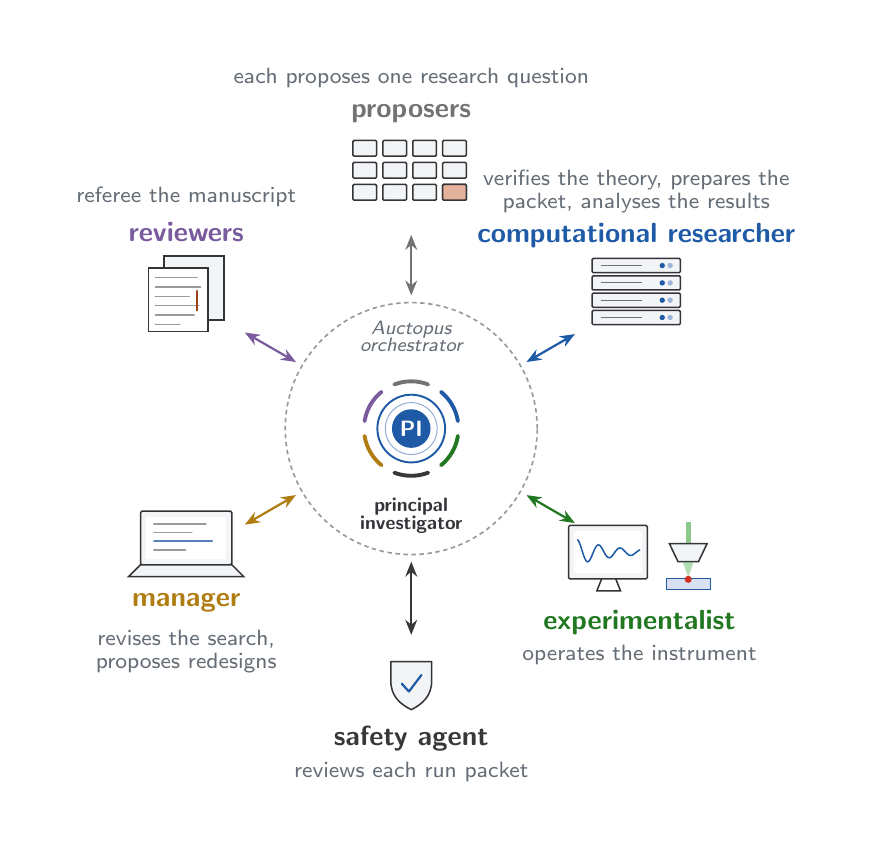
\begin{tikzpicture}[x=1mm, y=1mm,
  show background rectangle, inner frame xsep=5mm, inner frame ysep=4mm,
  background rectangle/.style={fill=cbg, rounded corners=3mm},
  ink/.style={draw=cink, line width=0.55pt},
  name/.style={font=\normalsize\bfseries, align=center},
  does/.style={font=\footnotesize, text=csub, align=center},
  spoke/.style={line width=0.8pt, {Stealth[length=1.9mm,width=1.5mm]}-{Stealth[length=1.9mm,width=1.5mm]}}]

\def\R{33}     % centre of each role's icon
\def\ring{16}  % the orchestrator

% ---------- the orchestrator: a ring around the PI, one spoke per role ----------
\draw[cring, line width=0.6pt, dash pattern=on 1.6pt off 1.3pt] (0,0) circle (\ring);
\node[does, font=\scriptsize\itshape, anchor=south] at (0,8.6) {Auctopus\\[-2pt]orchestrator};
\foreach \a/\c/\r in {90/cask/24.6, 30/cprove/24.0, -30/cmeasure/24.0, -90/csafe/26.2, -150/cdesign/24.4,
                      150/creviewc/24.4} {
  \draw[spoke, \c] (\a:\ring+0.9) -- (\a:\r);
}

% ---------- the principal investigator ----------
\foreach \a/\c in {90/cask, 30/cprove, -30/cmeasure, -90/csafe, -150/cdesign, 150/creviewc} {
  \draw[\c, line width=1.4pt, line cap=round] (\a-21:6.0) arc[start angle=\a-21, end angle=\a+21, radius=6.0];
}
\filldraw[draw=cblue, line width=0.7pt, fill=cpaper] (0,0) circle (4.3);
\draw[cblue!50, line width=0.35pt] (0,0) circle (3.3);
\fill[cblue] (0,0) circle (2.45);
\node[text=white, font=\footnotesize\bfseries, inner sep=0pt] at (0,0) {PI};
\node[name, text=ctext, font=\scriptsize\bfseries, anchor=north] at (0,-7.6) {principal\\[-1.5pt]investigator};

% ---------- proposers (top) ----------
\begin{scope}[shift={(90:\R)}]
  \foreach \i in {0,...,3} {\foreach \j in {0,...,2} {
    \filldraw[ink, fill=cfill, rounded corners=0.4pt] ({-7.4+\i*3.8},{-4.0+\j*2.8}) rectangle ++(3.0,2.0);
  }}
  \filldraw[ink, fill=corange!45, rounded corners=0.4pt] ({-7.4+3*3.8},{-4.0}) rectangle ++(3.0,2.0);
  \node[name, text=cask, anchor=south] at (0,4.6) {proposers};
  \node[does, anchor=south] at (0,9.0) {each proposes one research question};
\end{scope}

% ---------- computational researcher (upper right) ----------
\begin{scope}[shift={(30:\R)}]
  \foreach \k in {0,...,3} {
    \filldraw[ink, fill=cfill, rounded corners=0.4pt] (-5.6,{-3.3+2.2*\k}) rectangle (5.6,{-1.5+2.2*\k});
    \draw[cink!70, line width=0.35pt] (-4.5,{-2.4+2.2*\k}) -- (0.7,{-2.4+2.2*\k});
    \fill[cblue] (3.3,{-2.4+2.2*\k}) circle (0.34);
    \fill[cblue!45] (4.3,{-2.4+2.2*\k}) circle (0.34);
  }
  \node[name, text=cprove, anchor=south] at (0,5.2) {computational researcher};
  \node[does, anchor=south] at (0,9.6) {verifies the theory, prepares the\\[-1pt] packet, analyses the results};
\end{scope}

% ---------- experimentalist (lower right) ----------
\begin{scope}[shift={(-30:\R)}]
  \filldraw[ink, fill=cfill, rounded corners=0.5pt] (-8.6,-2.6) rectangle (1.4,4.2);
  \fill[cpaper] (-7.9,-1.9) rectangle (0.7,3.5);
  \draw[cblue, line width=0.55pt, domain=0:8.0, samples=60, smooth]
       plot ({-7.5+\x}, {0.8+1.6*exp(-0.2*\x)*cos(deg(2.3*\x))});
  \draw[ink] (-4.4,-2.6) -- (-5.0,-4.1) -- (-2.0,-4.1) -- (-2.6,-2.6);
  \fill[claser, opacity=0.55] (6.3,4.6) rectangle (6.9,1.9);
  \filldraw[ink, fill=cfill] (4.2,1.9) -- (9.0,1.9) -- (7.9,-0.4) -- (5.3,-0.4) -- cycle;
  \fill[claser, opacity=0.35] (5.9,-0.4) -- (7.3,-0.4) -- (6.6,-2.4) -- cycle;
  \filldraw[draw=cblue, line width=0.45pt, fill=cblue!18] (3.8,-3.9) rectangle (9.4,-2.5);
  \fill[cred!75!corange] (6.6,-2.65) circle (0.45);
  \node[name, text=cmeasure, anchor=north] at (0.4,-5.3) {experimentalist};
  \node[does, anchor=north] at (0.4,-9.8) {operates the instrument};
\end{scope}

% ---------- safety agent (bottom) ----------
\begin{scope}[shift={(-90:\R)}]
  \filldraw[ink, fill=cfill, line join=round] (-2.6,3.4) -- (2.6,3.4) -- (2.6,1.0)
       .. controls (2.6,-1.0) and (1.4,-2.0) .. (0,-2.7) .. controls (-1.4,-2.0) and (-2.6,-1.0) .. (-2.6,1.0) -- cycle;
  \draw[cblue, line width=0.8pt, line cap=round, line join=round] (-1.2,0.6) -- (-0.3,-0.4) -- (1.3,1.7);
  \node[name, text=csafe, anchor=north] at (0,-3.6) {safety agent};
  \node[does, anchor=north] at (0,-8.1) {reviews each run packet};
\end{scope}

% ---------- manager (lower left) ----------
\begin{scope}[shift={(-150:\R)}]
  \filldraw[ink, fill=cfill, rounded corners=0.5pt] (-5.8,-0.8) rectangle (5.8,6.0);
  \fill[cpaper] (-5.1,-0.1) rectangle (5.1,5.3);
  \foreach \y/\l/\c in {4.4/6.6/cring, 3.3/4.8/cring, 2.2/7.4/cblue!75, 1.1/4.0/cring} {
    \draw[\c, line width=0.6pt, line cap=round] (-4.1,\y) -- (-4.1+\l,\y);
  }
  \filldraw[ink, fill=cfill] (-7.3,-2.3) -- (7.3,-2.3) -- (5.8,-0.8) -- (-5.8,-0.8) -- cycle;
  \node[name, text=cdesign, anchor=north] at (0,-3.3) {manager};
  \node[does, anchor=north] at (0,-7.8) {revises the search,\\[-1pt] proposes redesigns};
\end{scope}

% ---------- reviewers (upper left) ----------
\begin{scope}[shift={(150:\R)}]
  \filldraw[ink, fill=cfill] (-2.8,-2.7) rectangle (4.8,5.4);
  \filldraw[ink, fill=cpaper] (-4.8,-4.2) rectangle (2.8,3.9);
  \foreach \y/\l in {2.7/5.3, 1.5/5.7, 0.3/4.3, -0.9/5.5, -2.1/4.9, -3.3/3.1} {
    \draw[cring, line width=0.55pt, line cap=round] (-3.9,\y) -- (-3.9+\l,\y);
  }
  \draw[corange!80!black, line width=0.7pt, line cap=round] (1.4,1.0) -- (1.4,-1.5);
  \node[name, text=creviewc, anchor=south] at (0,6.0) {reviewers};
  \node[does, anchor=south] at (0,10.4) {referee the manuscript};
\end{scope}

\end{tikzpicture}
\end{document}
